%%%%%%%%%%%%%%%%%%%%%%%%%%%%%%%%%%%%%%%%%%%%%%%%%%%%%%%%%%%%%%%%%%%%%%%%%%%%%
\section{Many-Core Architectures}\label{sec:back-manycore}
%%%%%%%%%%%%%%%%%%%%%%%%%%%%%%%%%%%%%%%%%%%%%%%%%%%%%%%%%%%%%%%%%%%%%%%%%%%%%
Till the beginning of this century, rapid growing rate of CPU frequency
has successfully pushed forward the high performance computing into
petascale. However, such improvement is not free, we had to pay for
increasing cost of per core power consumption that even raised up the
power wall ceasing any frequency growth. That is, any additional increase
in the power usage of a processor would result in the processor's components
melting or becoming extremely unreliable. Consequently, single processors
can no longer become faster, the only way to improve performance for
high-end processors is to add more cores and hardware threads.

Many-core architectures provides applications such massively parallel
environment and have already being successfully used in several most
powerful supercomputers in the world. For example, both the world's No.1 system,
Tianhe-2 developed by China's National University of Defense
Technology~\cite{tianhe2}, and the No.10 system, Stampede located at Texas
Advanced Computing Center~\cite{stampede} use the Intel Xeon Phi coprocessors
to accelerate their computation; Mira at Argonne National Laboratory, an IBM
BlueGene/Q supercomputer ranked at No.5 in the world, also forms as
many-core embedded platform~\cite{mira}.
In this section, we introduce the basic structure and programming
environment of two many-core productions.

\subsection{Intel Xeon Phi Coprocessor}

The Intel Many Integrated Core (MIC) architecture features a large amount
of CPU cores inside single chip with Linux-based operating system. It
provides applications a similar programming and execution environment
as the normal CPU systems, with supporting massive parallelism and vector
capability to achieve high floating-point performance. Different from
the GPU accelerators, the many-core chip can be run as both floating-point
accelerator, and a standalone system.

\begin{figure}[ht]
\centering
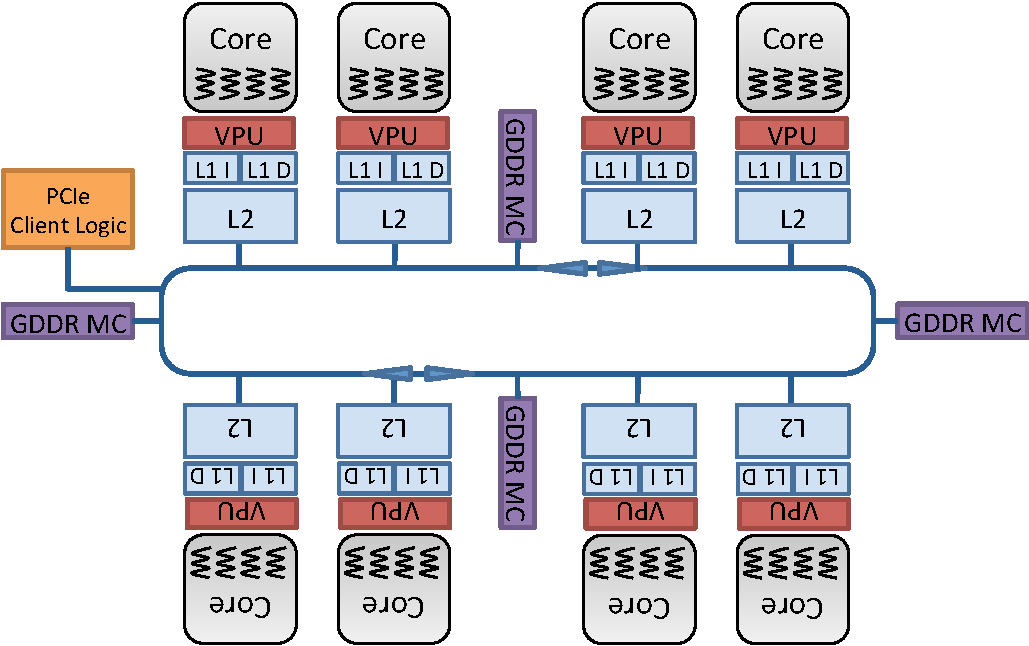
\includegraphics[width=1\textwidth]{figures/background/arch-mic-knc.pdf}
\caption{Knight Corner Chip Constriction.}
\label{fig:arch-mic-knc}
\end{figure}

Intel published the first commercial release of MIC architecture, codenamed
Knights Corner (KNC) in 2012~\cite{knc,mic}. It provides a minimum of 60
light-weight cores and separate GDDR5 memory embedded on single chip,
with each core capable of supporting four hardware threads and a 512-bit
SIMD vector processing unit (VPU). As shown in Figure~\ref{fig:arch-mic-knc},
all of the cores have fully private and coherent cache: 32~KB instruction
+ 32~KB data L1, and 512~KB L2 (unified), with high bandwidth bidirectional
ring interconnection. Eight dual-channel GDDR5 memory controllers (MC)
are symmetrically distributed on the ring to provide high bandwidth access
to the 8~GB or more GDDR5 memory from any cores.

The KNC coprocessors is usually connected with host CPU cores and inter-node
communication device (e.g., InfiniBand) via PCI-express on each computing
node of Xeon Phi based supercomputers as demonstrated in
Figure~\ref{fig:arch-mic-node}. For example, the Stampede
supercomputer~\cite{stampede} employs one KNC chip (SE10P) connected to
two Intel E5 8-core (Sandy Bridge) processors on each node; the Tianhe-2
supercomputer is constructed as three Xeon Phi chips with two Intel
Ive Bridge processors per computing node~\cite{tianhe2}.

The KNC provides three programming models for application
development: native, offload or symmetric. In the \emp{native mode}, KNC's
own micro-Linux operating system manages the on-chip resources and exposes
comprehensive system calls to support user programs running with both MPI
and threads parallelism. For some of the system calls that cannot be handled
directly on the KNC card are transparently forwarded to the host CPU and
returned with the result received from host after the execution.
Thus the applications can directly run on the KNC environment similar as
that on traditional CPU systems. With regard to the internal communication
between MPI processes,  processes located on the same card communicate
with each other through shared memory; processes on the same computing node
but located on two KNC cards communicate using the PCIe peer-to-peer
capabilities; for the communication outside the node, the capability of
direct data transfer without host intervention has been provided on some
networks such as InfiniBand. On the other hand, the \emp{offload mode}
offers the possibility of running as an accelerator like GPUs, and
the \emp{symmetric mode} can be used in MPI applications where processes
are distributed on both KNC and host CPUs. We only focus on the \emp{native
mode} in this thesis.

\begin{figure}[ht]
\centering
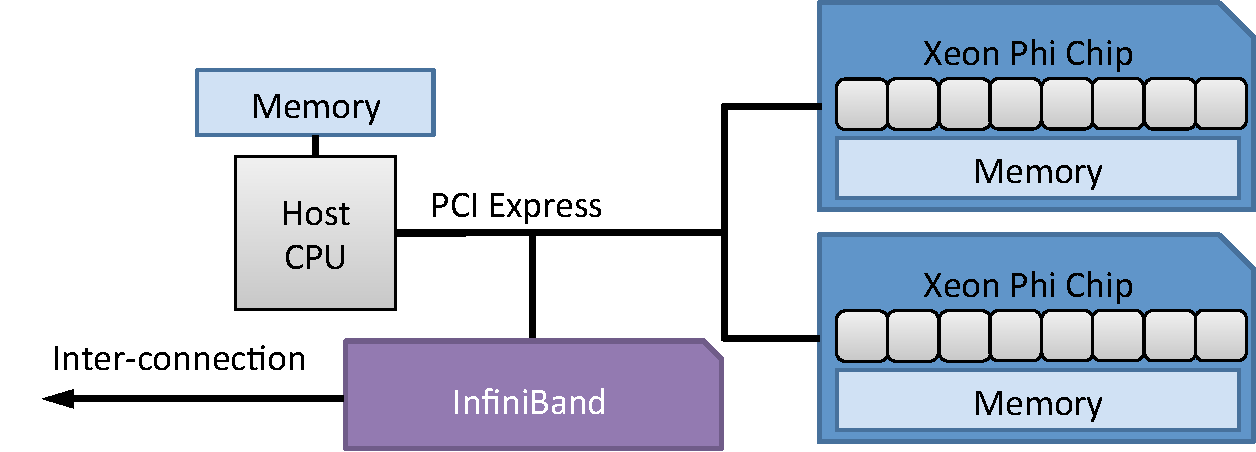
\includegraphics[width=0.8\textwidth]{figures/background/arch-mic-node.pdf}
\caption{Computing Node Structure on Xeon Phi supercomputers.}
\label{fig:arch-mic-node}
\end{figure}

Furthermore, Intel has recently also announced the details of its next
generation of the Xeon Phi product family, codenamed Knights Landing (KNL).
KNL is a fully self-hosted architecture that can offer applications the
standalone execution environment similar but more comprehensive compared
to the \emp{native mode} on KNC card. Greater than 60
cores with four hardware threads and two powerful VPUs each are embedded
on single chip with more complex but high bandwidth mesh interconnection.
This design allows 3x single thread performance compared to KNC and achieve
more than 3~TeraFlops peak performance per singe socket node. At least
two of the upcoming supercomputers, Cori at the National Energy Research
Scientific Computing Center (NERSC)~\cite{cori}, and Theta at Argonne National
Laboratory~\cite{theta}, have decided to be constructed using the KNL
processors. More detailed information of the KNL architecture can be found
at~\cite{knl}.

\subsection{Blue Gene/Q Supercomputer}

